\documentclass[journal,12pt,onecolumn,draftcls]{IEEEtran}
\usepackage{amsmath,amssymb,amsfonts}
\usepackage{algorithmic}
\usepackage{graphicx}
\usepackage{xcolor}
\usepackage{float}
\usepackage{setspace}
\usepackage{hyperref}
\hypersetup{
      colorlinks=true,
      linkcolor=blue,
      citecolor=black,      
      urlcolor=blue
}

\doublespacing

\begin{document}
\title{One Class Autoencoder for Anomaly Detection of Malaria Infected Cells}
\author{\IEEEauthorblockN{Author Name}}
\maketitle
\begin{abstract}
    Malaria is a major public health challenge, particularly in developing countries. Current diagnostic methods are limited in accuracy and efficiency, which motivates the need for more effective malaria detection methods. Anomaly detection is a promising approach, but the lack of sufficient abnormal instances is a major problem that limits the performance of available approaches. In this study, we propose a one class autoencoder that is trained on normal cell images to learn underlying patterns and identify deviations. Our proposed approach demonstrates high accuracy for the detection of malaria-infected cells in microscopic images, making it a promising solution for malaria detection.
\end{abstract}

\begin{IEEEkeywords}
anomaly detection, malaria detection, deep learning, one class autoencoders
\end{IEEEkeywords}

\section{Problem Statement}
Malaria is a life-threatening disease caused by parasites transmitted to people through the bites of infected mosquitoes. The World Malaria Report 2022 highlights that there were an estimated 247 million malaria cases in 2021 in 84 endemic countries \cite{who2022}, with most of the increase coming from countries in the WHO African Region. Malaria case incidence reduced from 82 in 2000 to 57 in 2019, before increasing to 59 in 2020, with no change in case incidence between 2020 and 2021. The increase in 2020 was associated with disruptions to services during the COVID-19 pandemic, which led to an estimated additional 13.4 million cases between 2019 and 2021, 29 countries accounted for 96\% of global malaria cases, with Nigeria, the Democratic Republic of the Congo, Uganda, and Mozambique accounting for almost half of all cases. The WHO African Region, with an estimated 234 million cases in 2021, accounted for about 95\% of global cases \cite{who2022}.

Malaria continues to pose a significant public health challenge, particularly in developing countries, where access to diagnostic tools and treatment can be limited. Current diagnostic methods for malaria detection, such as microscopy and rapid diagnostic tests \cite{wilson2012}, have several limitations, including variability in diagnostic sensitivity and specificity, high cost and dependence on skilled personnel. As such, the development of more accurate and efficient methods for malaria detection, particularly in resource-limited settings, is critical.

To address these challenges, we turn to anomaly detection, also known as outlier detection. It is a technique that is used to identify rare or unexpected observations or patterns in a dataset \cite{chandola2009}, \cite{ruff2021}, \cite{edgeworth1887}. It offers a promising avenue in the pursuit of improved malaria diagnostics. It is widely used in various fields, such as finance, cybersecurity, and medical diagnosis, where detecting anomalies is crucial for detecting fraud, identifying network intrusions, or diagnosing diseases. This concept has proven useful in identifying the presence of malaria virus in cell images.

In this research endeavor, we propose the utilization of a one class methodology for the classification of red blood cells depicted in microscopic images. It leverages normal cell images to solve a commonly encountered challenge in the medical field which is the insufficient number of abnormal or infected instances.

One class anomaly detection is a machine learning technique that is particularly useful for identifying anomalous instances within a single class of data. By training a model on a large and diverse dataset of normal instance, the proposed method should be able to extract deep features of the data that can distinguish normal from anomalous sets. These deep features can be learned using deep learning models, such as autoencoders and convolutional neural networks (CNNs), which are able to capture hierarchical representations of the data that include both global and local features in instances where images are used \cite{torres2021}.

Deep learning which falls under the umbrella of machine learning involves creating computer models that can teach artificial intelligence systems. What sets deep learning apart is its ability to automatically recognize important patterns in data without needing experts to manually choose the most relevant information. These features make deep learning especially useful in fields like medical imaging. In areas where it's tough to figure out which parts of an image matter, such as disease classification and tumor detection, deep learning models excel at making sense of complex data, making them a valuable tool in healthcare and beyond \cite{torres2021}.

In summary, the major solutions that this proposal seeks to solve are:
\begin{itemize}
    \item Address Inefficient Anomalous Data: It tackles the significant challenge of data scarcity in medical imaging by leveraging normal cell images to develop a robust detection model.
    \item Reduced False Positives: These methods often lead to fewer false positive detections, crucial in applications where false alarms can have serious consequences, such as medical diagnostics or fraud detection.
\end{itemize}

Through this research, we show that our approach demonstrates above-average accuracy for detecting infected cells in microscopic images using one class autoencoders. This makes our model a promising and reliable tool for improving malaria diagnosis and enhancing healthcare outcomes, particularly in resource-limited settings.

\section{Literature Review}
Bobde et al \cite{bobde2022} highlighted the use of an autoencoder algorithm as a solution to address the malaria cell classification problem. They employed the autoencoder model, training it with data and freezing the encoder for feature extraction. This extracted encoder was then integrated with fully connected CNN layers and utilized the softmax activation function for binary classification. The model underwent fine-tuning and was integrated into a user-friendly web application, showcasing its real-life applicability even for users with minimal training.

Autoencoders, an unsupervised learning algorithm, compress input data into a lower-dimensional code, reconstructing the output. Comprising encoder, code, and decoder components, they enable the discovery of coherent structures within input data, serving as a data-specific, lossy, and unsupervised dimensionality reduction tool. In this study, the autoencoder's encoder portion acted as a feature extractor, identifying crucial features in blood sample images for classification. The study also employed Convolutional Neural Networks (CNNs), inspired by biological processes, to analyze images. CNNs assign importance to features and capture spatial and temporal dependencies using relevant filters. Their deep architecture allows them to excel in image analysis.

During the training, validation, and testing phases, several metrics were recorded to assess the model's performance. These metrics included accuracy, loss, precision, recall, and F1 Score. Leveraging an EarlyStopping callback, the researchers minimized the risk of overfitting the model, optimizing computational resources. The results were impressive, with the model achieving a training accuracy of 96.06\%, a validation accuracy of 96.52\%, and a testing accuracy of 95.31\%. The training process spanned 84 epochs before halting due to the EarlyStopping callback, taking approximately 4 hours to complete. These metrics underscored the model's robustness and effectiveness in the context of malaria cell classification.

Musa et al \cite{musa2022} proposed a Convolutional Neural Network (CNN) for classifying malaria cells using blood image data, thereby indicating whether or not an individual has malaria. The model utilized a sixteen-layer CNN model, demonstrating remarkable efficacy, achieving an impressive average accuracy of 97.37\% during ten-fold cross-validation. Specifically, the model excelled in accurately classifying input images, boasting a high classification accuracy of 94\%.

The experimental phases of the Convolutional Neural Network (CNN) approach involved testing various activation functions and epochs to enhance accuracy. After comparing different combinations, the most effective configuration from the experiments utilized ReLU as the first activation function, sigmoid as the second, Adam as the optimizer, and 25 epochs, achieving an impressive accuracy of 95.6\%.

Reddy et al. \cite{reddy2021} developed a system integrating Inception v3, a Transfer Learning model, with an SVM classifier for malaria detection. In this configuration, Inception v3 played a pivotal role in extracting essential features for classification, which were subsequently used by the SVM classifier to make predictions. Inception v3, a component of Google's Deep Learning Architecture series, served as a potent Deep Convolutional Network.

The model was frozen up to its bottleneck layer, situated just below the fully connected layer. Throughout the training phase, the model demonstrated an impressive accuracy of 93\%. In the final testing stage, it achieved a remarkable accuracy of 94.8\%.

\section{Dataset}
In this proposal, our research framework is rooted in a compiled dataset obtained from Giemsa-stained thin blood smear slides \cite{chakradeo2020}. This dataset comprises samples sourced from 150 patients infected with P. falciparum and 50 healthy individuals, painstakingly collected at Chittagong Medical College Hospital, Bangladesh.

The cornerstone of our investigation is the Malaria Detection dataset, meticulously curated and sourced from IEEEDataPort, titled ``Malaria Dataset (Thin Blood Smear, Updated).'' Despite its value, the dataset posed a challenge due to a considerable number of inaccurately labeled images. To address this, a review and relabeling process was undertaken. Consequently, the images were restructured into several groups with two pivotal categories: uninfected and parasitized.

Additionally, as part of our broader dataset utilized for the deep learning model, we incorporated a secondary dataset sourced from Kaggle into our research \cite{kaggle}. This Kaggle dataset includes two classes of uninfected cells (RBCs and leukocytes) and four classes of infected cells (gametocytes, rings, trophozoites, and schizonts). Annotators were allowed to mark some cells as difficult if not clearly in one of the cell classes. The data exhibited a notable imbalance, with uninfected RBCs being predominant, constituting over 95\% of all cells.

For the kaggle dataset model training, we capitalized on the provided bounding box coordinates. These coordinates were instrumental in precisely cropping and categorizing cells into two primary groups: uninfected and infected. This step allowed us to focus specifically on regions of interest within the images and streamlining the training process.

\begin{figure}[H]
\centering
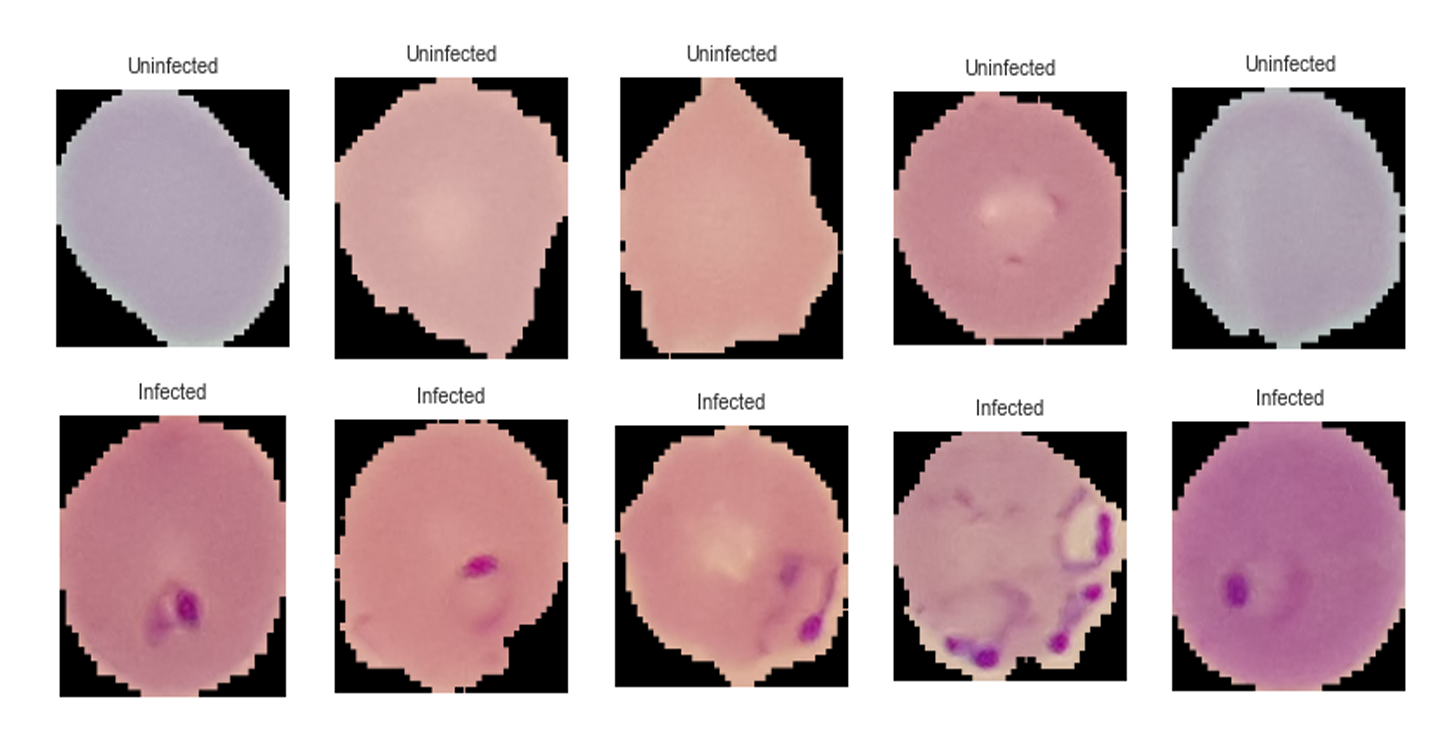
\includegraphics[width=0.8\textwidth]{images/fig1.png}
\caption{Dataport Infected and Uninfected Cell Images.}
\label{fig:fig1}
\end{figure}

\begin{figure}[H]
\centering
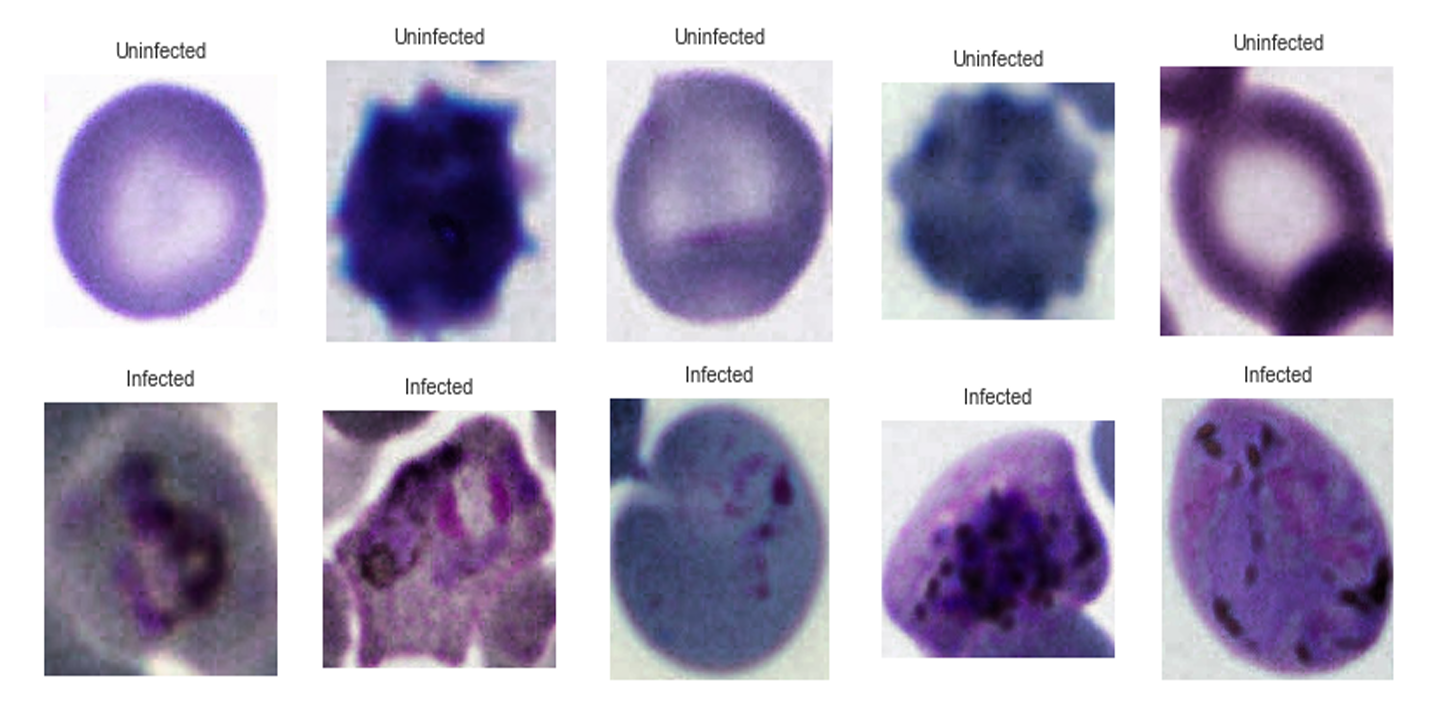
\includegraphics[width=0.8\textwidth]{images/fig2.png}
\caption{Bounding Box Infected and Uninfected Cropped Cell Images.}
\label{fig:fig2}
\end{figure}

\section{Proposed Method}
In this research, we introduce a novel approach utilizing a one class convolution autoencoder designed specifically to learn a compressed representation of input images belonging to a single class, in this case, microscopic images of malaria cells. The unique characteristic of this type of autoencoder lies in its training objective: to reconstruct its input with minimal error. One class autoencoders are particularly valuable for anomaly detection, as they excel at identifying inputs that deviate significantly from the training data.

Our proposed autoencoder consists of three main components: an encoder, a latent space, and a decoder. In the encoder phase, the input data, representing the microscopic images of malaria cells, undergoes processing to transform it into a lower-dimensional representation, commonly known as a latent space or encoding. This encoding captures the essential features of the input data while significantly reducing its dimensionality. The latent space representation ideally captures the most salient features of normal data, and during training, the autoencoder learns to map normal data points to a specific region within this latent space.

\begin{figure}[H]
\centering
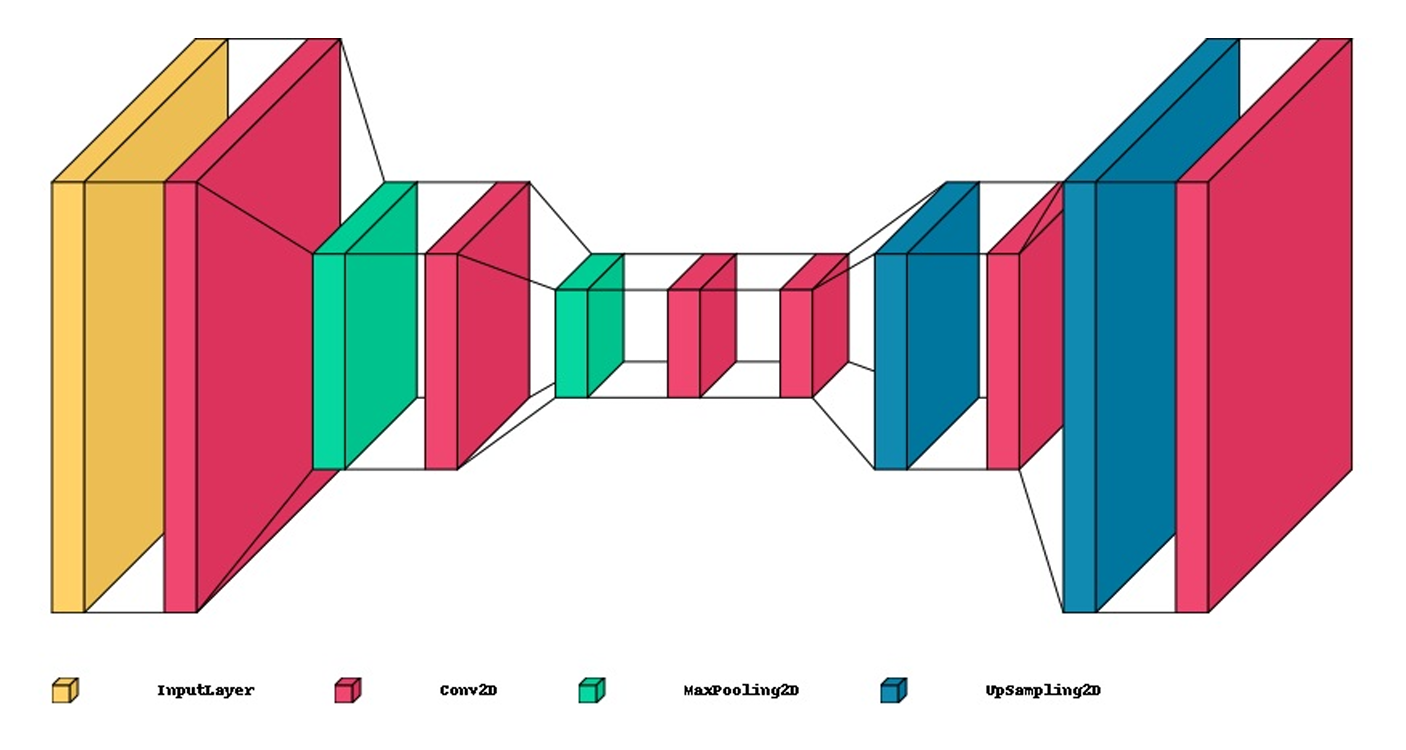
\includegraphics[width=0.8\textwidth]{images/fig3.png}
\caption{Reconstruction of Uninfected Cell Images using an Autoencoder.}
\label{fig:fig3}
\end{figure}

Following the encoder, the decoder, the second part of the network, attempts to reconstruct the input data from the encoding. The goal of the decoder is to generate output that closely resembles the original input, completing the reconstruction process. To quantify the quality of this reconstruction, we employ the mean squared error (MSE) as the loss function:

\begin{equation}
MSE = \frac{1}{N}\sum_{i=1}^{N}(x_i - y_i)^2
\end{equation}

where $N$ represents the total number of samples, $x_i$ is the actual value of the $i$-th sample, and $y_i$ is the predicted value of the $i$-th sample \cite{pu2012}.

During training, the model aims to minimize this loss, ensuring that the reconstructed outputs align closely with the inputs.

It is important to note that during the training phase, the one class autoencoder is exclusively exposed to normal, non-anomalous data. It learns to accurately reconstruct this normal data, and the latent space representations are shaped based on the distribution of this normal data. As a result, the model becomes adept at capturing the inherent patterns within normal cell images.

As a means of evaluation, we utilize the Structural Similarity Index (SSIM), enabling an understanding of the similarity between the original and reconstructed images. During the testing phase, SSIM scores offer a quantitative measure of the similarity between the unknown class samples and the known class data. Higher SSIM scores indicate a closer resemblance between the reconstructed and original images, providing valuable insights into the quality of the model's reconstructions \cite{fu2017}.

According to Wang et al \cite{wang2009} the original SSIM methodology is rooted in the understanding that the human visual system excels at extracting structural information from visual scenes. In the context of assessing image fidelity, preserving this structural detail is crucial. To differentiate between distortions, SSIM distinguishes between structural and nonstructural alterations. Nonstructural distortions, such as changes in luminance, contrast, gamma distortion, and spatial shifts, result from environmental or instrumental factors during image acquisition and display. These alterations don't affect the inherent structures of visual objects in the scene. Conversely, structural distortions, including additive noise, blur, and lossy compression, significantly impact the object structures within images.

The SSIM approach takes inspiration from the human visual system, treating it as an ideal information extractor capable of recognizing objects amidst various distortions. Thus, SSIM prioritizes sensitivity to structural distortions while automatically compensating for nonstructural ones. The SSIM index evaluates local image patches (denoted as x and y) from two compared images. It measures similarities in patch luminances (l(x, y)), local patch contrasts (c(x, y)), and local patch structures (s(x, y)). These similarities are quantified using easily computed statistics, which are then combined to form the local SSIM index (S(x, y)).

The SSIM formula, while seemingly complex, breaks down into manageable components:

\begin{equation}
SSIM(x, y) = \frac{(2\mu_x\mu_y + C_1) + (2\sigma_{xy} + C_2)}{(\mu_x^2 + \mu_y^2 + C_1)(\sigma_x^2 + \sigma_y^2 + C_2)}
\end{equation}

Here, $\mu_x$ and $\mu_y$ represent local sample means, $\sigma_x$ and $\sigma_y$ are local sample standard deviations, $\sigma_{xy}$ is the sample cross-correlation of x and y after mean removal, and $C_1$, $C_2$, and $C_3$ are small positive constants preventing numerical instability.

The SSIM index exhibits symmetry (S(x, y) = S(y, x)) and is bounded within the range of -1 to 1. A score of 1 indicates perfect similarity between the compared patches. The index operates within a sliding window, yielding a SSIM map, and the overall image SSIM score is computed, often by averaging SSIM values across the image. Adaptive space-variant weighting and scale-based computations enhance its performance across various spatial scales.

In our approach, classification decisions are made using a predefined SSIM threshold, which is derived from the acceptable false negative rate (FNR). To establish this threshold, we utilize the validation set and the reconstructed images obtained from the autoencoder. We plot a bar graph of the validation set, comparing the SSIM-based reconstruction errors of normal and anomalous images. By analyzing this graph, we determine a threshold value where the majority of the normal images have reconstruction errors above the threshold.

For each test sample, its SSIM-based reconstruction error is calculated. If the reconstruction error is above the determined threshold, the sample is classified as belonging to the normal class. Conversely, if the error falls below the threshold, the sample is identified as part of the anomalous class. This method ensures that the classification decision is based on a statistically significant criterion, enhancing the accuracy of the classification process.

Correspondingly, with a predefined threshold $\varepsilon$, the known and unknown classes can be discriminated by:

\begin{equation}
x_t \in \begin{cases} 
\text{known class,} & \text{if } \varepsilon_t < \varepsilon \\
\text{unknown class,} & \text{otherwise}
\end{cases}
\end{equation}

Note that the threshold $\varepsilon$ is typically defined based on the tolerable false negative rate (FNR) by users or practitioners.

In summary, our proposed method leverages the power of a one class autoencoder, training it to learn and reconstruct normal microscopic images of malaria cells. Through this approach, we enable the model to effectively identify anomalous or infected instances during the anomaly detection phase, showcasing the potential of our method in enhancing malaria diagnosis accuracy.

\begin{figure}[H]
\centering
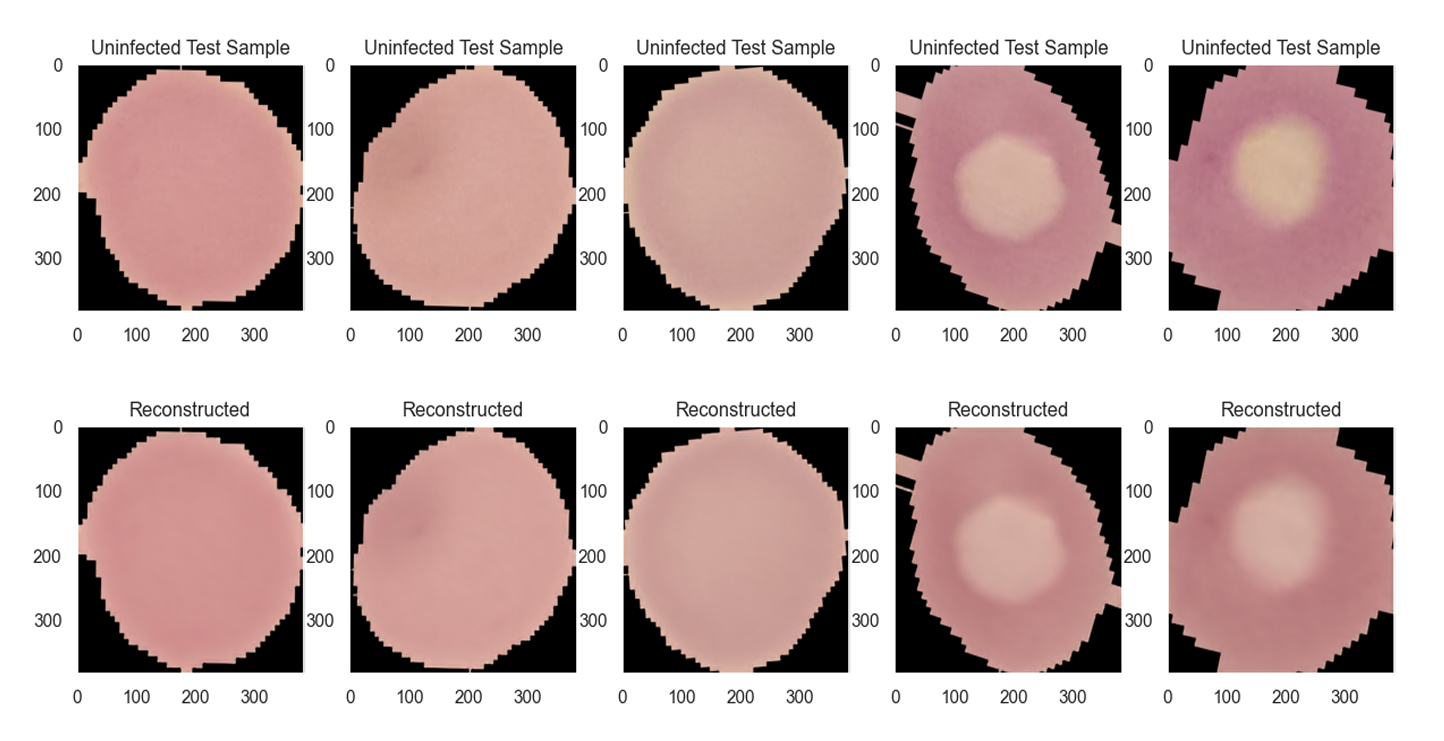
\includegraphics[width=0.8\textwidth]{images/fig4.png}
\caption{Reconstruction of Dataport IEEE Dataset Uninfected Cell Images using an Autoencoder.}
\label{fig:fig4}
\end{figure}

\section{Results}
Evaluating the viability of our proposed method is an essential part of a research study. Metrics are used to evaluate the proposed model and to understand how well our model performs. The metrics we used include:

\begin{figure}[H]
\centering
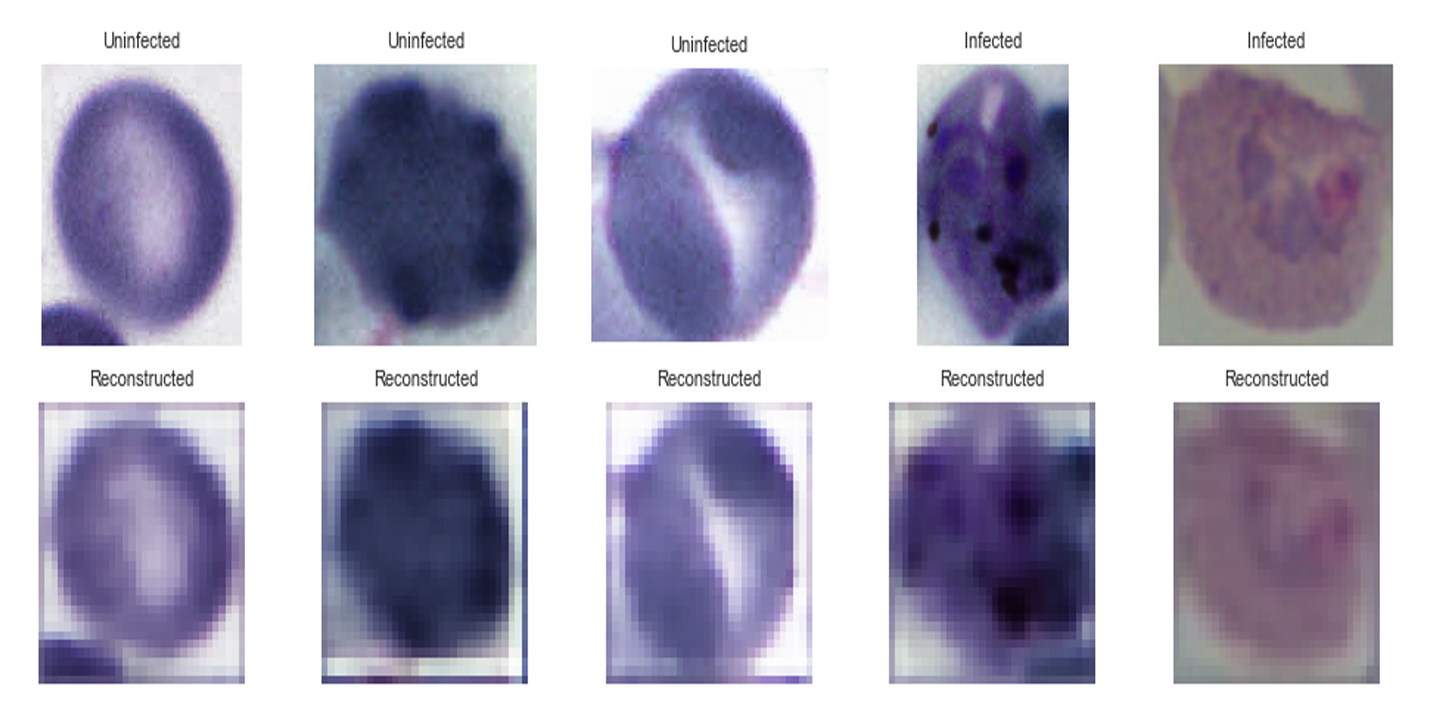
\includegraphics[width=0.8\textwidth]{images/fig5.png}
\caption{Reconstruction of Bounding Box Dataset Cell Images using an Autoencoder.}
\label{fig:fig5}
\end{figure}

SSIM: Leveraging SSIM as an evaluation metric aligns with our goal of capturing both global and local features in the reconstructed images. By emphasizing perceptual similarity, our approach provides a more comprehensive assessment of the model's ability to preserve critical visual information during the reconstruction process. This integration of SSIM and thresholding enhances the precision and reliability of our method in classifying malaria-infected cells in microscopic images, making it a robust tool for accurate medical diagnosis and analysis.

Our attention was drawn towards comparing and identifying a useful evaluation metric in terms of classifying both normal and abnormal cell images with high accuracy and a very low false positive rate and as such we evaluated our model's classification capabilities using both MSE and SSIM.

MSE gave very poor results when it comes to classifying malaria images and this was evidenced by the research done by Wang et al \cite{wang2009} who illustrated the weakness of MSE and the strengths of SSIM in terms of using them as evaluation metris.

According to Wang et al \cite{wang2009} MSE when used as an evaluation metric, although it works best as a loss function, it displays various setbacks as follows:

Lack of Sensitivity to Human Perception: MSE does not accurately reflect how humans perceive differences in visual perception. It treats all pixel errors equally, ignoring the fact that some errors are more perceptually significant than others. For instance, small errors in smooth areas might be less noticeable to the human eye than similar errors in textured or high-contrast regions. The failure to account for these perceptual differences leads to inaccurate assessments of image fidelity.

Inability to Capture Structural Information: Images often contain structural elements such as edges, textures, and patterns, which are vital for human perception. MSE treats images as a collection of independent pixels and fails to capture these structural relationships. Changes in these relationships, even if pixel values remain the same, can significantly impact perceived image quality.

Failure to Address Image Content-Dependent Variations: MSE treats all pixels equally, regardless of their perceptual importance. In many images, certain regions (e.g., faces in portraits) are more critical for perception than others. MSE's uniform treatment of pixels does not consider these variations in perceptual importance.

Neglect of Error Signal Characteristics: MSE does not consider the characteristics of the error signal, such as its correlation with the original image or the signs of error signal samples. In real-world scenarios, errors are often correlated with the image content, and their signs can influence visual perception. MSE's uniform treatment of all errors disregards these critical factors.

These characteristics are towered by the efficient ways that SSIM sees, perceives and evalutes images and errors and these include:

Luminance Comparison: SSIM calculates the luminance term by comparing the average pixel intensity of the two images. It considers how the overall brightness of the images relates to each other. If the average pixel intensity of two images is similar, it implies a similarity in luminance.

Contrast Comparison: The contrast term is calculated by comparing the standard deviation of pixel intensities. It measures the variation in pixel intensity. Images with similar contrast will have a smaller difference in their standard deviations, indicating a similarity in contrast.

Structure Comparison: The structure term assesses the correlation between pixel intensities of the images. It considers how the pixels are arranged relative to each other. If the pixels in corresponding positions are correlated, it suggests a similarity in structure.

These underlying principles made SSIM the best placed method as an evaluation metric and gave better results. We evaluted the model based on these metrics.

Accuracy: This metric measures the overall correctness of the model's predictions. A higher accuracy indicates better performance. A higher accuracy value, closer to 1.0 or 100\%, suggests that the model is making more correct predictions and is generally desirable \cite{powers2011}.

Recall: Recall, also known as sensitivity or true positive rate, is a metric that measures the ability of a classification model to correctly identify all relevant instances in a dataset. In the context of our research, recall quantifies the proportion of actual positive instances (malaria-infected cells) that our model correctly identified. Missing an infected cell (a false negative) could have significant consequences, especially in medical contexts. Therefore, maximizing recall for the positive class (infected cells) is crucial \cite{powers2011}.

Precision: Precision measures the accuracy of the positive predictions made by the model. It quantifies the proportion of correctly predicted positive instances out of all instances predicted as positive \cite{powers2011}.

F1 Score: The F1 score is a metric that combines both precision and recall into a single value. Precision measures the accuracy of the positive predictions made by the model, while recall measures the model's ability to capture all the positive instances in the dataset. The F1 score is the harmonic mean of precision and recall and provides a balance between these two metrics \cite{powers2011}.

Specificity: Specificity measures the proportion of actual negative instances (non-infected cells, in the case of malaria detection) that the model correctly identifies as negative. It focuses on the ability of the model to avoid false alarms by correctly classifying negative instances \cite{powers2011}.

\subsection{Evaluation Metrics Results}
The autoencoder, although not delivering optimal results initially, displayed effectiveness in minimizing loss throughout the training period spanning 35 epochs. The decreasing trend in loss values signifies the model's ability to reduce the disparity between input and output images. This outcome indicates a successful compression of input data while preserving vital features. Notably, the training process remained stable, showing no signs of overfitting; this stability was evidenced by the validation loss following a consistent downward trajectory similar to the training loss. Despite the initial challenges, these results mark a foundation upon which improvements can be built, illustrating a pathway toward refining the model's performance.

The confusion matrix analysis highlighted some challenges with the Mean Squared Error (MSE) metric. Specifically, it showed that the MSE-based struggled in accurately distinguishing between infected and uninfected cells in malaria detection. As depicted in the confusion matrices, MSE consistently exhibited higher rates of false positives and false negatives compared to the Structural Similarity Index (SSIM). This indicated that MSE failed to capture the subtle visual nuances crucial for identifying malaria-infected cells, leading to misclassifications in both directions. In contrast, SSIM, which evaluates structural patterns, luminance, and contrast differences, proved to be more adept at capturing the essential features in the images. This shows that the model employing SSIM as a metric demonstrated superior accuracy and reliability in malaria detection, making it the preferred choice for this critical task.

Our model has achieved exceptional results, demonstrating outstanding performance on both the Bounding Boxes Kaggle Malaria dataset and the IEEE Dataport Malaria Dataset. Despite the challenges faced, our model showcased a remarkable true positive rate, with a recall of 0.97 for the Bounding Boxes Kaggle Malaria dataset and an even higher 0.99 for the IEEE Dataport Malaria Dataset. These results instill confidence in the model's ability to identify malaria-infected cells and inspire optimism for future enhancements.

\begin{figure}[H]
\centering
\begin{minipage}{0.45\textwidth}
  \centering
  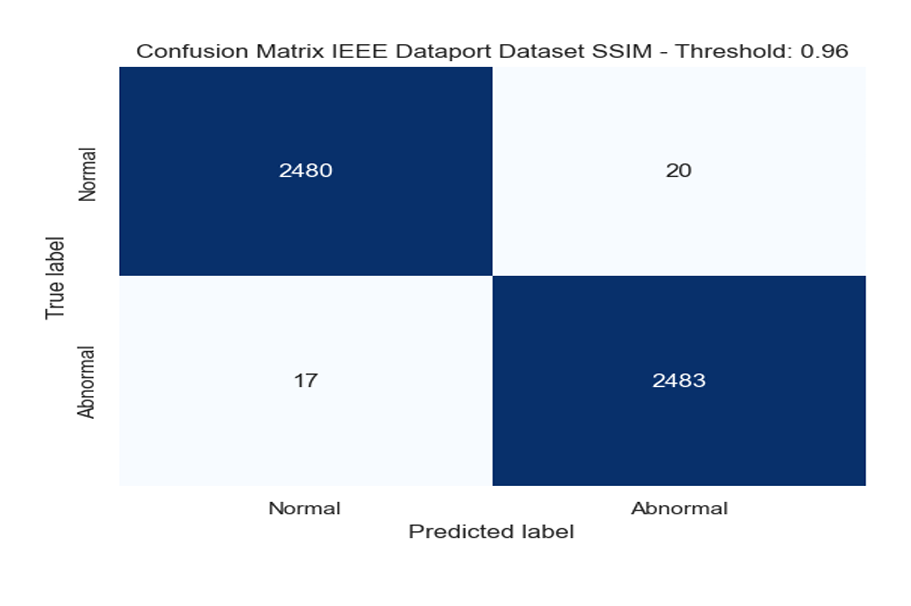
\includegraphics[width=\textwidth]{images/fig6.png}
  \caption{SSIM Confusion Matrix threshold 0.96}
  \label{fig:fig6}
\end{minipage}\hfill
\begin{minipage}{0.45\textwidth}
  \centering
  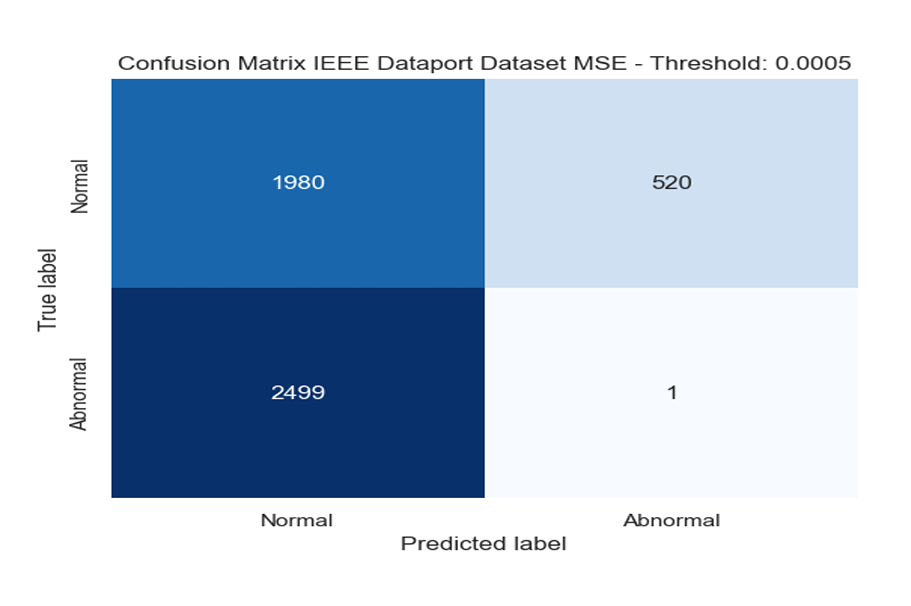
\includegraphics[width=\textwidth]{images/fig7.png}
  \caption{MSE Confusion Matrix threshold 0.0015}
  \label{fig:fig7}
\end{minipage}
\end{figure}

\begin{figure}[H]
\centering
\begin{minipage}{0.45\textwidth}
  \centering
  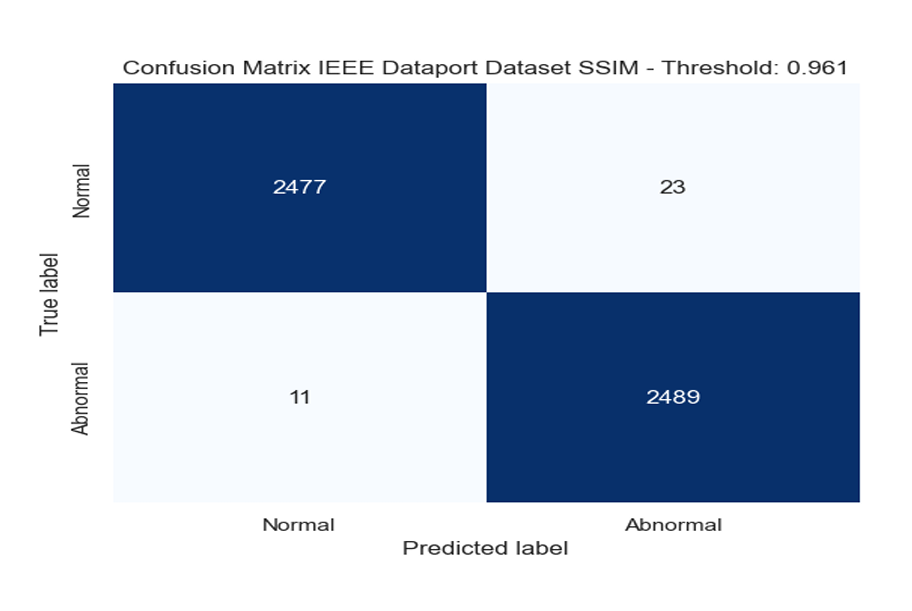
\includegraphics[width=\textwidth]{images/fig8.png}
  \caption{SSIM Confusion Matrix threshold 0.961}
  \label{fig:fig8}
\end{minipage}\hfill
\begin{minipage}{0.45\textwidth}
  \centering
  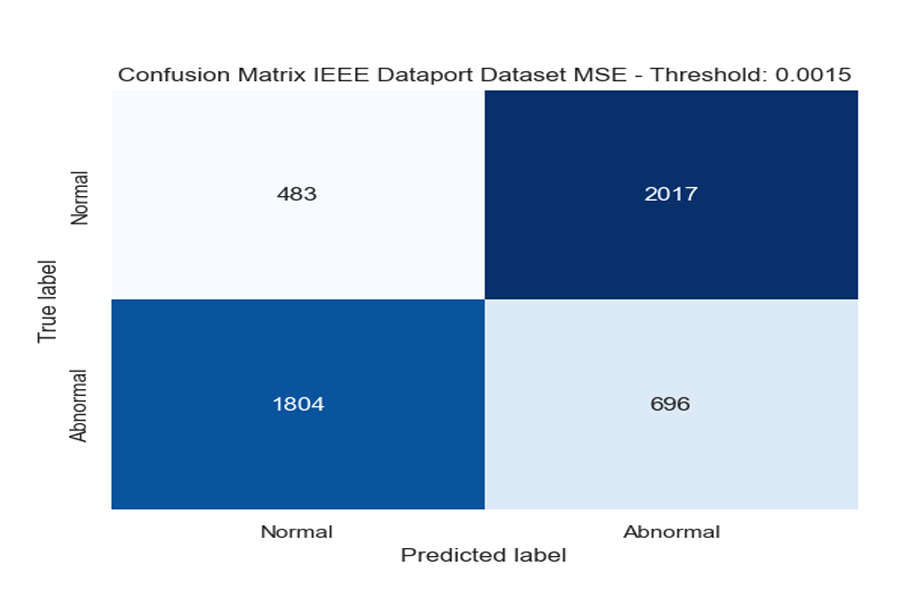
\includegraphics[width=\textwidth]{images/fig9.png}
  \caption{MSE Confusion Matrix threshold 0.0025}
  \label{fig:fig9}
\end{minipage}
\end{figure}

\begin{figure}[H]
\centering
\begin{minipage}{0.45\textwidth}
  \centering
  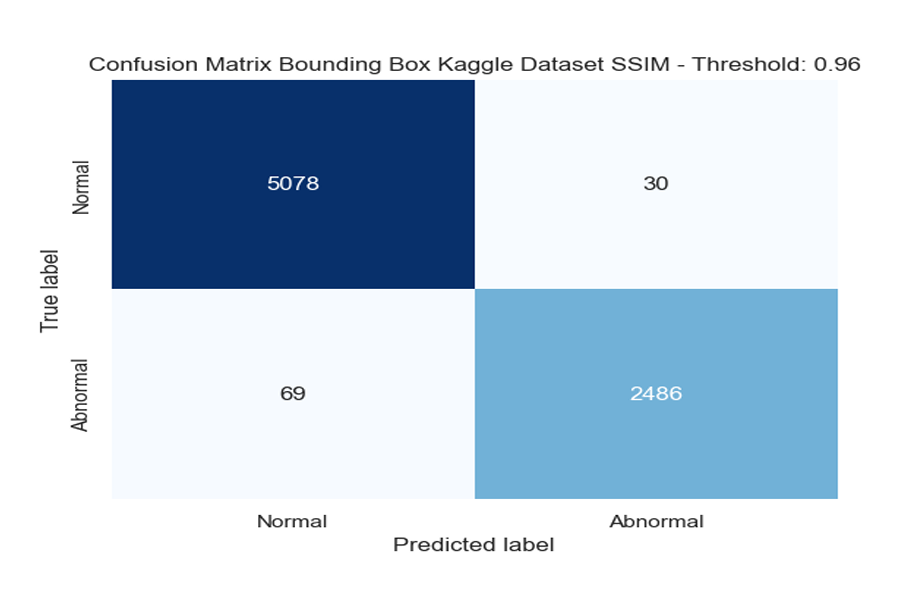
\includegraphics[width=\textwidth]{images/fig10.png}
  \caption{SSIM Confusion Matrix threshold 0.96}
  \label{fig:fig10}
\end{minipage}\hfill
\begin{minipage}{0.45\textwidth}
  \centering
  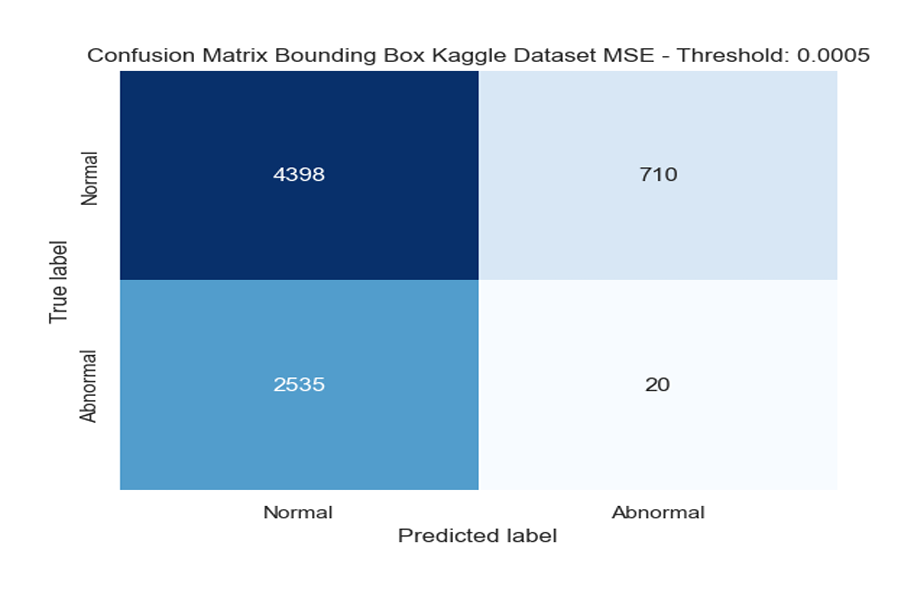
\includegraphics[width=\textwidth]{images/fig11.png}
  \caption{MSE Confusion Matrix threshold 0.0035}
  \label{fig:fig11}
\end{minipage}
\end{figure}

\begin{figure}[H]
\centering
\begin{minipage}{0.45\textwidth}
  \centering
  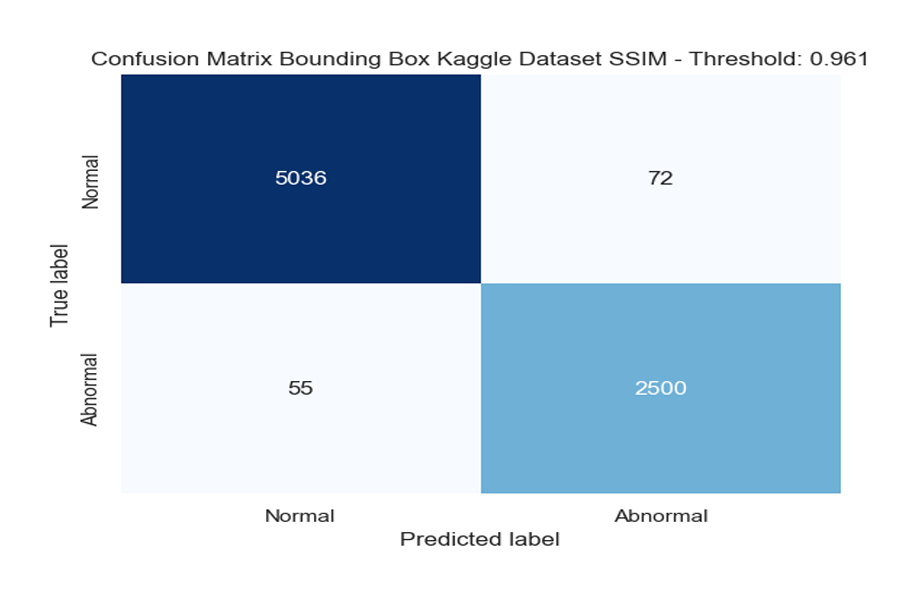
\includegraphics[width=\textwidth]{images/fig12.png}
  \caption{SSIM Confusion Matrix threshold 0.961}
  \label{fig:fig12}
\end{minipage}\hfill
\begin{minipage}{0.45\textwidth}
  \centering
  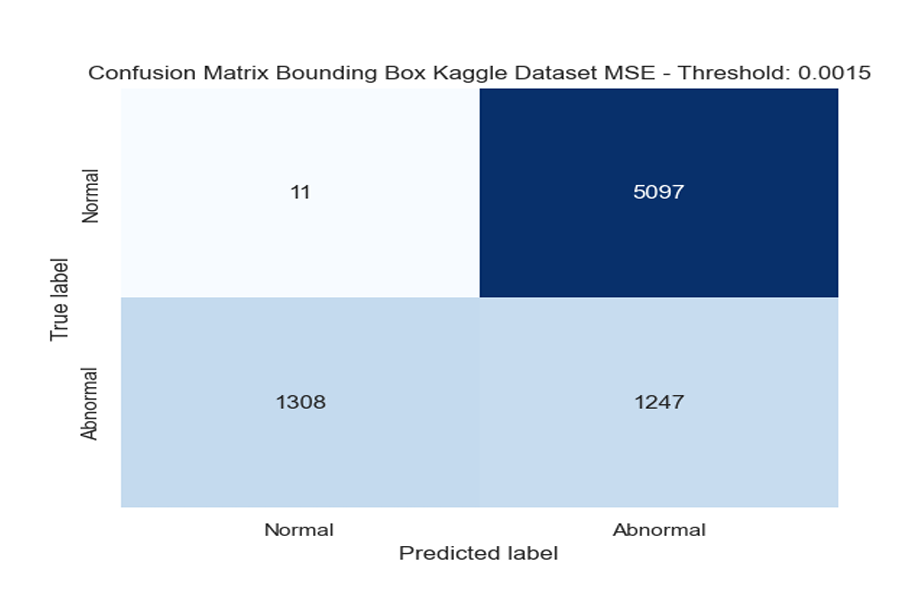
\includegraphics[width=\textwidth]{images/fig13.png}
  \caption{MSE Confusion Matrix threshold 0.0045}
  \label{fig:fig13}
\end{minipage}
\end{figure}

\begin{figure}[H]
\centering

\includegraphics[width=\textwidth]{images/fig14.png}
\caption{SSIM and MSE Confusion Matrices}
\label{fig:fig14}
\end{figure}

The precision of 0.99 for both datasets is a testament to the model's accuracy in positive predictions. Notably, the recall for abnormal instances is outstanding, with values of 0.97 for the Bounding Boxes Kaggle Malaria dataset and 0.99 for the IEEE Dataport Malaria Dataset. These results indicate that a high percentage of actual abnormal instances were correctly identified, with 97\% for the former and an impressive 99\% capture rate of true positives for the latter.

The F1-score, considering both precision and recall, reflected a balanced and exceptional performance for both datasets, with values of 0.98 and 0.99 for the Bounding Boxes Kaggle Malaria dataset and the IEEE Dataport Malaria Dataset, respectively. These metrics highlight the model's proficiency in effectively classifying both normal and abnormal instances.

The overall accuracy of the model at 0.99 underscores its consistently high performance across datasets. These outstanding results are a testament to the model's capabilities.

\subsection{Threshold Identification}
In this research, the determination of the SSIM threshold value was an important aspect of the process, it involved the analysis of the validation set. Plotting the validation data provided a visual representation of the distribution of normal instances. By selecting a threshold value where all the normal instances were consistently clustered, a balanced approach was achieved. This method allowed for the optimization of the true positive rate while minimizing false positives.

It is crucial to emphasize that the performance of any model is intricately linked to the specific dataset and context in which it is employed. The parameters utilized in this study were carefully chosen considering the size of the dataset under examination. It's worth noting that when dealing with larger sample sizes, different parameters might be necessary to ensure optimal performance. The selection of an appropriate SSIM threshold value is a pivotal step in the anomaly detection process, as it directly impacts the model's ability to distinguish between normal and abnormal instances. A threshold set too high might lead to overlooking anomalies (false negatives), while a threshold set too low could result in misclassifying normal instances as anomalies (false positives). Therefore, the methodology employed in this study, involving careful plotting and selection, aimed to strike a balance between sensitivity and specificity, ensuring the model's reliability in real-world applications.

\begin{figure}[H]
\centering
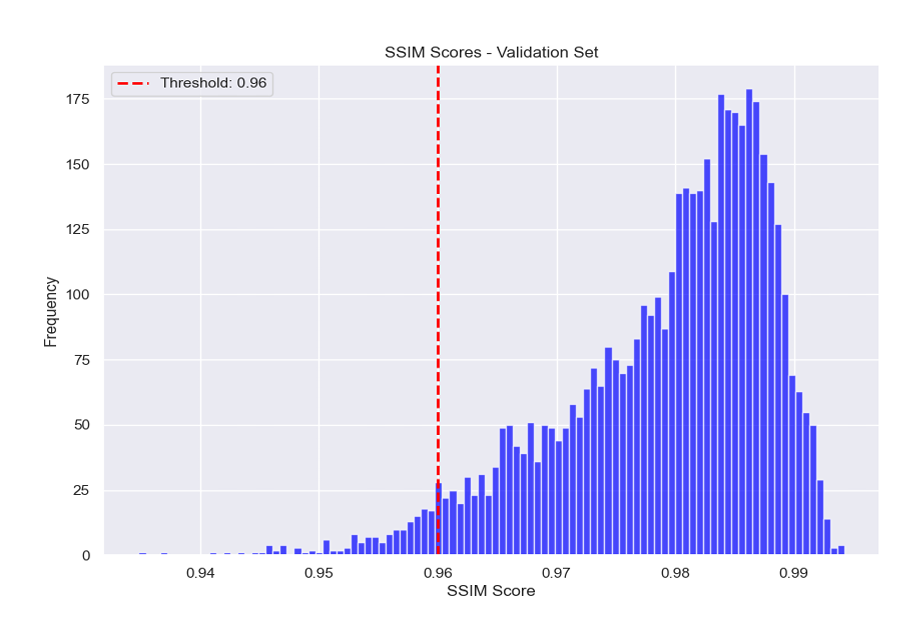
\includegraphics[width=\textwidth]{images/fig15.png}
\caption{SSIM Threshold Selection IEEE Dataport Dataset, threshold here chosen above 0.96}
\label{fig:fig15}
\end{figure}

\begin{figure}[H]
\centering
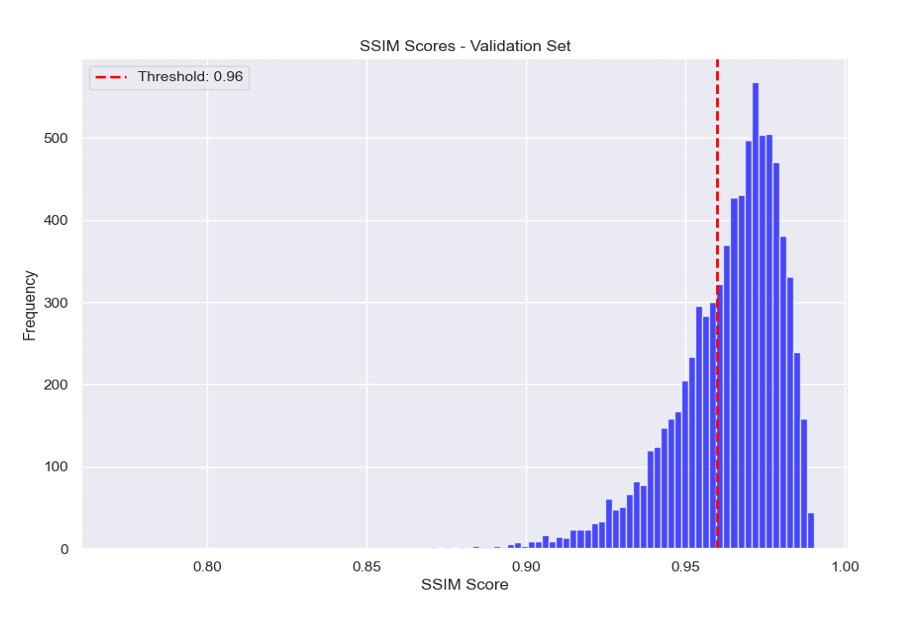
\includegraphics[width=\textwidth]{images/fig16.png}
\caption{SSIM Threshold Selection Bounding Box Kaggle Dataset, threshold here chosen above 0.96}
\label{fig:fig16}
\end{figure}

\begin{table}[H]
    \centering
    \label{table:eval_metrics}
    \begin{tabular}{l|c|c|c|c|c}
    \multicolumn{6}{c}{\textbf{TABLE I}} \\
    \multicolumn{6}{c}{\textbf{EVALUATION METRICS}} \\
    \hline
    Model & OC & Autoencoder & CNN & Transfer & OC \\
     & Autoencoder & & & Learning & Autoencoder \\
     & (IEEE & & & & (Bounding \\
     & Dataport) & & & & Boxes Data) \\
    \hline
    Accuracy & 0.99 & 0.9531 & 0.9728 & 0.948 & 0.99 \\
    Recall (Sensitivity) & 0.99 & 0.9528 & 0.9515 & - & 0.97 \\
    Specificity & 0.99 & - & 0.9962 & - & 0.99 \\
    Precision & 0.99 & 0.9626 & 0.9960 & - & 0.99 \\
    F1-score & 0.99 & 0.9577 & 0.9732 & - & 0.98 \\
    \hline
    \end{tabular}
    \end{table}

\section{Conclusion}
Malaria is a life-threatening disease, so early diagnosis can save lives. The accuracy of diagnosing malaria from blood smears relies on the efficiency of medical professionals and the quality of instruments used in the diagnostic process. This can put a heavy strain on medical professionals in rural areas with less medical facilities. Deep learning methods with high accuracy in diagnosing the disease can alleviate this strain on the healthcare system and make the diagnostic process easier and faster. The proposed method can prove to be an effective medical diagnosis aid.

In addition, the proposed method; a one class autoencoder, helps solve the issue that most models face which is lack of enough abnormal instances. This is because the autoencoder is trained on a dataset of normal images, and then learns to identify abnormal images by finding images that are different from the normal images. This means that the autoencoder can be trained on a relatively small dataset of normal images, and still be able to identify abnormal images with high accuracy.

\newpage
\bibliographystyle{IEEEtran}
\bibliography{references}
\end{document}